%
%  $Description: Author guidelines and sample document in LaTeX 2.09$
%
%  $Author: ienne $
%  $Date: 1995/09/15 15:20:59 $
%  $Revision: 1.4 $
%

\documentclass[times, 10pt,twocolumn]{article}
\usepackage{latex8}
\usepackage{times}
\usepackage{balance}
\usepackage{epsfig}
\usepackage{graphicx}
%\usepackage{wrapfig}

%\documentstyle[times,art10,twocolumn,latex8]{article}

%-------------------------------------------------------------------------
% take the % away on next line to produce the final camera-ready version
\pagestyle{empty}

%-------------------------------------------------------------------------
\begin{document}

\title{Beyond The Kiss-Cam: Measuring The Fan Using Computer Vision-based Analytics}

\author{George Williams  \hspace{0.1in} Christoph Bregler \hspace{0.1in} Ian Spiro \hspace{0.1in} Christoph Bregler \\
\emph{Dept. of Computer Science, Courant Institute, New York University}\\
\emph{george,chris,ian@movement.nyu.edu}\\
% For a paper whose authors are all at the same institution,
% omit the following lines up until the closing ``}''.
% Additional authors and addresses can be added with ``\and'',
% just like the second author.
%\and
%Second Author\\
%Institution2\\
%First line of institution2 address\\ Second line of institution2 address\\
%SecondAuthor@institution2.com\\
}

\maketitle
\thispagestyle{empty}

\begin{abstract}
What are fans really doing at the game?  When are they watching the action on the field/court, and when are they buried in their phone or tablet ?  Which ads do they notice on the JumboTron, and which ones do they ignore ?  Who’s joining in the “wave” and who’s not?  Are they having fun ?

If you are a club trying to retain seat-buying fans, fill empty chairs, or effectively use an advertising budget, then these are important questions to answer.

Video surveillance can be a useful tool here, but in and of itself cannot scale to large stadium crowds.  In this paper, we describe a method that applies vision-based techniques to surveillance footage.  Our method attempts to measure stadium fan engagement and sentiment, via body gesture- and action-recognition, and to measure visual attention, via estimated gaze.  We combine both machine learning algorithms and inexpensive, crowd-sourcing techniques to achieve speed and scale.  Moreover, we show how its possible to preserve the anonymity of the fans during the analysis.

We experimented using crowd footage at a college basketball game and 
\end{abstract}



%-------------------------------------------------------------------------
\Section{Introduction}
%-------------------------------------------------------------------------
\section{Related Work}
\label{sec_related}
%-------------------------------------------------------------------------
\section{Approach}

\subsection{Data Collection: Game Day}
\label{sec_GameDay}

We set up 4 HD cameras at a college basketball game and positioned them above the audience at balcony level.  We aimed 3 cameras at the most populated areas of the stands.  The camera views did not overlap.  We manually adjusted the zoom so that we captured as many fans as possible in each view, but not so far zoomed-out that each face spanned no less than around 12 pixels.  Any less than 12 pixels and the performance of the software-based face detector decreases significantly [REF].  We aimed the final camera at the basketball game and adjusted the zoom to capture the action at both ends of the court, including the scoreboard which hovered above the center of the court.  Figure XX shows 3 of the camera views.

\begin{figure}[bt]
\centering
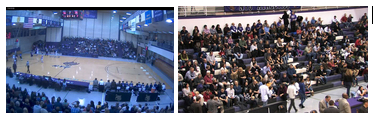
\includegraphics[width=0.46\columnwidth]{cams}
\caption{\label{fig_example_mos} \small Examples of Motion Signatures.  The green colored signature shows how the orientation of the sparse flow features changes over time (top row), and the red-blue color coded signature shows the delta features (middle row).}
\end{figure}

\subsection{MOS: Motion Orientation Signatures}
\label{sec_MOS}

\subsection{Face Tracking and Grid based Coarse Locality}

\subsection{GMM-Super-Features}
\label{sec_superfeat}

\subsection{Discriminant Classification}

\subsection{Comparison with Bag-Of-Feature Architectures}
\label{sec_relatedbag}

\section{Multi-Modal Experiments}

Figure \ref{fig_examples}  shows some example video frames from our database.  In total we have 72 minutes of video data with $320 \times 240$ pixel resolution. For each subject we have at least 4 different video clips recorded at different times.   Most subjects are public figures like international politicians or talk show hosts.  We are currently also collecting a database of ``non-famous'' people.

\section{Discussion}


\section{Acknowledgements}
We would like to thank Peggy Hackney, Ian Spiro, Andreas Stolcke, Yann LeCun, and Rob Fergus for useful discussions and pointers, and the Office of Naval Research (ONR N000140910076, N000140910789).


%-------------------------------------------------------------------------
{\tiny
\bibliographystyle{latex8}
\bibliography{vision}
}
\end{document}

